\vspace{0.5cm}

Se añaden los métodos de asignación y obtención a la clase \textit{persona}.

\subsection*{persona.hpp}
\begin{lstlisting}
/* NEW CODE */
    int Asignar_Nombre(std::string elNombre);
    int Asignar_Fecha_Nacimiento(int Anio, int Mes, int Dia);
    int Asignar_Lugar_Origen(std::string Lugar);


    std::string Obtener_Nombre();
    int Obtener_Anio_Nacimiento();
    int Obtener_Mes_Nacimiento();
    int Obtener_Dia_Nacimiento();
    std::string Obtener_Lugar_Origen();
/* NEW CODE */
\end{lstlisting}

\subsection*{persona.cpp}
\begin{lstlisting}
/* NEW CODE */
int persona::Asignar_Nombre(std::string elNombre)
{
    if( !Nombre )
    {
        Nombre = new std::string( elNombre );
        return 0;
    }

    std::cout << "El Nombre ya fue asignado" << std::endl;
    return 1;
}

int persona::Asignar_Fecha_Nacimiento(int Anio, int Mes, int Dia)
{
    if( !Fecha_nacimiento )
    {
        Fecha_nacimiento->tm_year = int( Anio );
        Fecha_nacimiento->tm_mon = int( Mes ) - 1;
        Fecha_nacimiento->tm_mday = int( Dia );
        return 0;
    }

    std::cout << "La Fecha de Nacimiento ya fue asignada" << std::endl;
    return 1;
}

int persona::Asignar_Lugar_Origen(std::string Lugar)
{
    if( !Lugar_nacimiento )
    {
        Lugar_nacimiento = new std::string( Lugar );
        return 0;
    }

    std::cout << "El Lugar de Nacimiento ya fue asignada" << std::endl;
    return 1;
}
/* NEW CODE */

/* NEW CODE */
std::string persona::Obtener_Nombre()
{
    if( Nombre )
        return *Nombre;
    return "Nombre no asignado";
}


int persona::Obtener_Anio_Nacimiento( )
{
    if( Fecha_nacimiento )
        return Fecha_nacimiento->tm_year;
    return 0;
}

int persona::Obtener_Mes_Nacimiento( )
{
    if( Fecha_nacimiento )
        return Fecha_nacimiento->tm_mon;
    return 0;
}

int persona::Obtener_Dia_Nacimiento( )
{
    if( Fecha_nacimiento )
        return Fecha_nacimiento->tm_mday;
    return 0;
}

std::string persona::Obtener_Lugar_Origen()
{
    if( Lugar_nacimiento )
      return *Lugar_nacimiento;
    return "Lugar de Nacimiento no asignado.";
}

/* NEW CODE */
\end{lstlisting}

Ya con esto, se modifica el archivo \texttt{class02.cpp} agregando un ejemplo que utilize los nuevos métodos:
\begin{figure}[H]
	\centering
	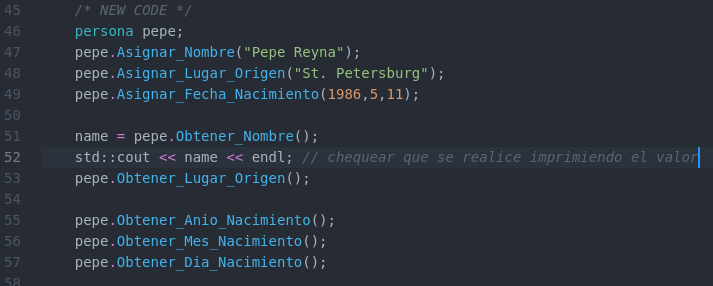
\includegraphics[scale=0.5]{./img/class02.png}
	\caption{Archivo \texttt{class02.cpp} modificado con un nuevo ejemplo "pepe".}
	\label{class02}
\end{figure}


\begin{figure}[H]
	\centering
	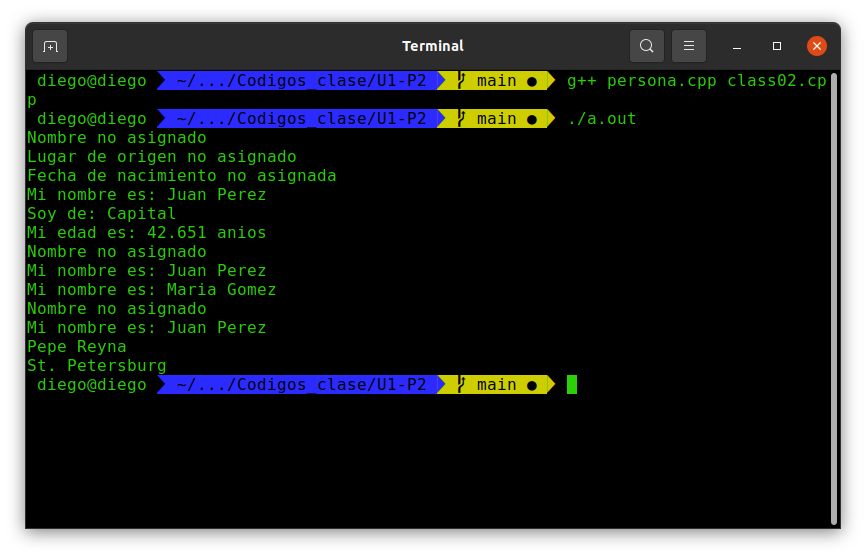
\includegraphics[scale=0.35]{./img/output.png}
	\caption{Output del programa con lo añadido.}
	\label{class02}
\end{figure}
